\documentclass{beamer}

\usepackage[utf8]{inputenc}
\usepackage{listings}
\usepackage{color}

\usepackage[english]{babel}
\usepackage{csquotes}
\usepackage{hyperref}
\usepackage{xcolor}
\usepackage{array}
\usepackage{amssymb}

\usepackage{graphicx}
\graphicspath{ {images} }

\usetheme{Madrid}
\usecolortheme{beaver}


%Information to be included in the title page:
\title{Implementing Dynamic Metadata in C\#}
\author{Paweł Łabno}
\institute{Seville More Helory}
\date{SFIonline webdev 2021}

\AtBeginSection[]
{
  \begin{frame}
    \frametitle{Table of Contents}
    \tableofcontents[currentsection]
  \end{frame}
}

\lstdefinestyle{sharpc}{language=[Sharp]C, frame=non, rulecolor=\color{blue!40!black}}

\begin{document}
\lstset{style=sharpc, linewidth=11cm, basicstyle=\ttfamily\footnotesize}

\frame{\titlepage}

\begin{frame}
\frametitle{Table of Contents}
\tableofcontents
\end{frame}

\begin{frame}
\frametitle{About speaker}

\begin{columns}
\begin{column}{0.3\textwidth}
 
\includegraphics[width=3cm, height=4cm]{photo.jpg}
\end{column}
\begin{column}{0.7\textwidth}  %%<--- here
	  \begin{itemize}
	  \item Senior Software Developer @ Seville More Helory
	  \item Graduated @ Jagiellonian University \& AGH 
	  \item Former Microsoft Student Partner
	 \item pawellabno1992@gmail.com
	\end{itemize}
\end{column}
\end{columns}


\end{frame}

\begin{section}{Introduction}

\begin{frame}

\frametitle{What is "metadata"}
\begin{displayquote}
data that provides information about other data
\end{displayquote}

\url{https://en.wikipedia.org/wiki/Metadata}

\end{frame}

\begin{frame}
\frametitle{Problem description}
Business scenario:
\\
You are developing Movie database with complete information about that movie including: \pause actors, production team, postproductions, other people involved, recording locations \& dates. \pause
That data would be later processed by Your partners Data Analysts to prepare movies people will love most.
\end{frame}

\begin{frame}
\frametitle{Business requirement - records preview}
\begin{tabular}{| m{0.5cm} | m{3.25cm} | m{1cm} | m{2.25cm} | m{1cm} | m{1.5cm} |}
\hline
No. &  Movie & Year & Locations & BO (bn \$) & Director \\
\hline \hline
1 & Avengers: Endgame & 2019 & USA,  Ireland & 2.798 & Russo Brothers \\ \hline
2 & Avatar & 2009 & USA,  New Zeland & 2.79 & James Cameron \\  \hline
3 & Titanic & 1997 & Canada, Mexico & 2.195 & James Cameron \\  
\hline
\end{tabular}

\end{frame}

\begin{frame}
\frametitle{Technical requirements}
Technical requirements for our solution: \pause
\begin{enumerate}
	\item Our application should be written in C\# \pause
	\item Application should be portable \pause
	\item Some updates could be done after few seconds \pause
	\item Our system should be easy to extend
\end{enumerate}
\end{frame}

\begin{frame}
\frametitle{Technical specification}
\begin{enumerate}
	\item We will use .NET 5 to build application \pause
	\item We will use not-relational database approach to make easier extension in future \pause
	\item For purposes of this session we will use InMemoryDatabase
\end{enumerate}
\end{frame}

\begin{frame}
\frametitle{Standard approach}

\lstinputlisting[firstline=12, lastline=17]{standard_movie.cs}

\end{frame}


\begin{frame}
\frametitle{Standard approach description}
In standard solution we are developing well-defined classes (e.g. Actor or Director) with specified all properties. 
There is a little risk that variable wouldn't be understood by developer. However adding new metadata type would be implementing
completely new class (maybe with little reusage of other components). Adding new property would always require software developer work.

\end{frame}

\begin{frame}
\frametitle{Pros \& cons of standard approach}

\begin{center}

\begin{tabular}{ | m{5.2cm} |  m{5.2cm} | }

\hline
 pros & cons \\ 
\hline \hline
Standard format of data, easily to learn & Very hard to extend, each new feature require implementing new class and properties \\  
\hline
 "Harder" to break system with invalid data/configuration & Unable to extend by business team / admin \\
\hline
Integration require knowledge about components and relations & \\ 
\hline
Exploration of data "column by column" & \\
\hline

\end{tabular}

 \pause \textbf{Extending requires devteam work}

\end{center}

\end{frame}

\end{section}


\begin{section}{Dynamic project concept}

\begin{frame}
\frametitle{Dynamic metadata concept}

In dynamic metadata approach we treat metadata and its configuration as a metadata with standard. E.g. in our movie database scenario metadata could be "Director" or "Actor" both storing some information about that person and \/ or her/his role in movie production. Adding new metadata kind would require just add new definition to database. 
\newline
\newline
In overall in that case development team will provide solution with definitions, values and property types. 

\end{frame}

\begin{frame}
\frametitle{Metadata definition}

What that object should contains?\\

\begin{itemize}
	\item Identifier or key
	\item Names to easily select by user
	\item Collection of properties
		\begin{itemize}
			\item Identifier or key
			\item Name
			\item Type
			\item Default value
		\end{itemize}
	\item Validators
		\begin{itemize}
			\item Cross-property validation configuration
			\item Context validation configuration
		\end{itemize}
\end{itemize}

\end{frame}

\begin{frame}
\frametitle{Metadata definition - code example}


\lstinputlisting[firstline=8, lastline=15]{MovieDatabase/MovieDatabase/Model/DynamicMetadata.cs}

\end{frame}

\begin{frame}
\frametitle{Metadata definition - key points}

\begin{enumerate}
	\item Type specifications
	\item Validation pipelines, middlewares, complex scenarios
	\item Cross-property \& cross-item validations
	\item Default values \& configuration
\end{enumerate}

\end{frame}

\begin{frame}
\frametitle{Metadata definition - possible bad solutions}

\begin{enumerate}
	\item Not specified type or trying to generalize some data
	\item Passing complete configuration to target object (e.g. Movie)
	\item Creating on database layer "tree-kind" structures
	\item Validators on property level (on database, it could be fine for front-end validation)
\end{enumerate}

\end{frame}

\begin{frame}
\frametitle{Metadata usage}
How should we extend default Movie class to better match our solution? \newline \newline \pause  In our project there should be new list of properties storing information about metadata. Each of this object should contains value and metadata definition and ... \pause that's all :)
\end{frame}

\begin{frame}
\frametitle{Sample request}

\lstinputlisting[firstline=2, lastline=21]{request.json}

\end{frame}

\begin{frame}
\frametitle{Sample request - 2nd Part }
On previous slide You could saw that "Value"  had three different data types assigned to field. With little work we could allow to this flexibility, however there is a hidden cost - we have to validate data passed in requests.

\end{frame}

\begin{frame}
\frametitle{Layers separation} 
Standard ASP.NET Core project is divided into three layers \pause
\begin{enumerate}
	\item Presentation \pause
	\item Business logic \pause
	\item Data access \pause
\end{enumerate}

Proper storage of data and communication with outer world is crucial for our problem.
\end{frame}

\begin{frame}
\frametitle{Parsing input data}


 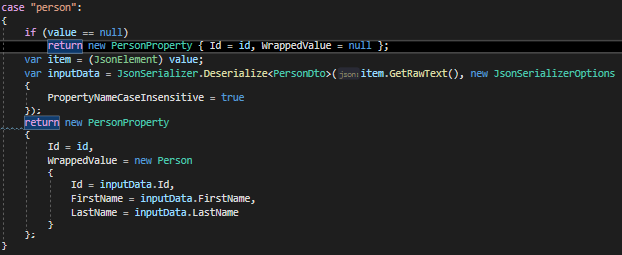
\includegraphics{personParsing.png}

\end{frame}


\end{section}

\begin{section}{Data validation \& concepts}

\begin{frame}
\frametitle{Data consistency}
For data analysis it is required to data be consistent in context of whole ecosystem. Since our data would be dynamic there are few additional issues that system should handle and in few following slides we will discuss data aspects. \newline \newline
System should be sure that if data is described as \textit{Person} that it contains person information, not numeric one.
\end{frame}

\begin{frame}
\frametitle{Constant up-do-date aspect}
To help processing data in system, developers should prepare solution that would keeps data up-to-data and having all actual information. To achieve that point they should prepare proper event handler, and when definition would change then all \textit{"Movies described with that description"} should be updated too. \newline
\newline
This topic we will continue in next section.

\end{frame}

\begin{frame}
\frametitle{Validation pipeline}
During creation of new metadata entry or updating existing one we should run validation process to  item. Since all configuration is stored in MetadataDefinition object we will generate validator based on that part of code. Validation process by default is invoked in context including \textit{Movie} and \textit{MetadataProperty}.
\end{frame}

\begin{frame}
\frametitle{Validation pipeline - algorithm flow}
\begin{enumerate}
	\item Create validator for MetadataDefinition
		\begin{enumerate}
			\item Find all validator configurations for definition
			\item For each validator
				\begin{enumerate}
					\item Get new instance of specified validator
					\item Set validation parameters
					\item Add validator to composite validator
				\end{enumerate}
			\item Return composite validator
		\end{enumerate}
	\item Validate item using validator
		\begin{enumerate}
			\item For each validator
				\begin{enumerate}
					\item Run validation on (metadata, movie) context
					\item Add errors to result collection
				\end{enumerate}
			\item Return list of all errors
		\end{enumerate}
	\item If validator returns any error - throw validation exception
\end{enumerate}
\end{frame}

\begin{frame}
\frametitle{IValidation interface}

\lstinputlisting{MovieDatabase/MovieDatabase/Services/Validation/IValidator.cs}

\end{frame}

\begin{frame}
\frametitle{Property validators}
This is the simplies kind of validator - we process just property data - e.g. we could check if year is in range or if connected user exists in proper database collection.
\end{frame}

\begin{frame}
\frametitle{Cross property validators}
This is a little more complex validator - in that case it is crucial that properties are properly named (we should use unique keys). In that case system will process a bit bigger chunk of data.

\end{frame}

\begin{frame}
\frametitle{Cross-items validators}
For example we want to have just one director for movie or ensure that actor really exist.
\end{frame}

\begin{frame}
\frametitle{Missing data}
This is first serious problem system should handle. First part of that issue could be handled by adding/removing/updating all properties updated in definition but there is another case. \newline \pause
What if property doesn't exist in request? \pause E.g. for actor we specify person but we don't specify character? \pause
System should create missing properties and then validates content or returns missing property exception.
\end{frame}

\begin{frame}
\frametitle{Duplicated property}
Another serious problem - \pause What if we are victims of somebody bad trying to break our system with invalid data? \pause \newline
There are three available solutions - You could select best matching Your requirements \pause \newline
\begin{enumerate}
	\item Handle just first occurance of property \pause
	\item Update property with each occurance \pause
	\item Raise an error
\end{enumerate}
\end{frame}

\begin{frame}
\frametitle{Additional property}
Next serious problem - \pause What if breaker from previous slide would add additional properties? \pause \newline
There are two available solutions - You could select best matching Your requirements \pause \newline
\begin{enumerate}
	\item Ignore that property \pause
	\item Raise an error
\end{enumerate}
\end{frame}

\begin{frame}
\frametitle{Invalid data type}
Final problem is with data stored in property and there could be two issues with that \pause
\begin{enumerate}
	\item Specified property type differs from type in definition - \pause we have person when it should be string \pause
	\item Data has invalid format and couldn't be parsed \pause
\end{enumerate}
\pause
\textbf{In that case it would be better to return error}
\end{frame}

\end{section}

\begin{section}{Definition versioning}

\begin{frame}
\frametitle{Definition versioning - Introduction}
Sometimes would be required to change definition in many ways, but all of them will affect how our system works. We should prepare our system for: 
\pause
\begin{itemize}
	\item Adding or removing property \pause
	\item Complete deletion of metadata definition \pause
	\item Changing type or default value \pause
	\item Changing validation configuration \pause
\end{itemize}
And we will discuss all of these cases in following slides
\end{frame}

\begin{frame}
\frametitle{Handling changes}
One of the biggest advantage of \textit{NoSQL} databases (e.g. MongoDB or CosmosDB) is that we don't keep explicite relations between objects. For the future discussion we will name Metadata definition as Source and Movie metadata as Target. \newline \newline

We should implement asynchronous update with Service Bus (Azure Service Bus or RabbitMQ) with event dispatched each time we change of definition (or at least with published change). On Target side we should implement handler to keep data up to date. \pause  \newline\textbf{NOTE: It could take several seconds to update data in Target entities}.

\end{frame}

\begin{frame}
\frametitle{Adding or removing property}
After adding or removing property in source object natural operation is updating target object in similar way.
\newline
It would be nice to set default value for newly created properties.
\newline
Removing property on source object should be implemented very carefully since we could break validation. We should handle also all validators connected to this property or block removal in case of any validators connected
\end{frame}

\begin{frame}
\frametitle{Deletion of metadata definition}
After confirmation of delete on purpose and dispatching event we have two acceptable options to implement: 
\begin{itemize}
	\item Delete items created with definition from DB
		\begin{itemize}
			\item We will have clean database without deleted items
		\end{itemize}
	\item Mark items as deleted 
		\begin{itemize}
			\item In that case data could be visible to users (but marked as deleted, not updatable) or invisible, but in that case we should handle deleted items each time (and users could be confused by lack of some items)
		\end{itemize}
\end{itemize}
Remember that it would be better to mark items as deleted rather than deleting them permanently. 
\end{frame}

\begin{frame}
\frametitle{Type or default value change}
Data definition could be hard to handle in many cases since we will have validators attached to these properties. Simlary to content of previous slide we could block these kind of changes or invalidate existing validator.
\newline
In case of type change system should update data with provided converter - implemented by software development team - or mark it out of date and require action by some administrator. 
\newline
In case of default value change we could simply iterate over collection of items and for properties marked with default value set new value. This would require add new property \textbf{IsDefaultValue} to dynamic property. 

\end{frame}

\begin{frame}
\frametitle{Configuration change}
The best solution in case of change of validator configuration would be process all data created basing on definition. Each instance with failed validation status we should mark as out of date. 

\end{frame}

\begin{frame}
\frametitle{Metadata history - definition}
It could be helpful to track changes in definition object. However this would require some changes into our code: \pause
\begin{itemize}
	\item We should create new object "DefinitionVersion" with unique Id, but referencing by key/id to MetadataDefinition \pause
	\item In MetadataDefinition we should store published version of item, with reference to it \pause
	\item There should be new endpoint to "Create new Definition Version" \pause
	\item All operations regarding changes in Definitions should have additional parameter "VersionId" \pause
	\item All "DefinitionChanges" Events should be handled only after publication of new version \pause
\end{itemize}
\end{frame}

\begin{frame}
\frametitle{Metadata history - movie}
I imagine that sometimes it would be nice to keep history of changes of Movie object. Since we could have two sources of changes for "Movie" object it wouldn't be so easy to implement similar solution as in scenario. We could simply create new object version for each time we change object - eg. add new metadata or we update metadata definition. But after little amount of time we could learn that we have one huge object (if we store information in one object) or we have a lot of big objects (in case we store each version separately). \pause
\newline
\begin{center}
	\textbf{Neither of these options is good for me}
\end{center}
\end{frame}

\begin{frame}
\frametitle{Change as commit}
There is design that would allows us to store many of changes with only one stored final object (to greatly simplify calculations). \newline \pause
But we should start with  ...  \pause GIT \newline \pause
We could treat each change (regardless type of these changes) as an operation - e.g. we will have operation to add new dynamic metadata, add new property or change value - each of these could be simplyfied to atomic (in context of system) operation. \newline
Each \textit{Save or publish} click would invoke processing of several atomic operations - like commit includes list of changes made inside files.  \newline
In this solution (recommended but hardest) We don't store full objects but we store changes.
\end{frame}

\begin{frame}
\frametitle {EventSourcing}
There is design pattern called \href{https://martinfowler.com/eaaDev/EventSourcing.html}{EventSourcing} in which we store operations (Events). In specified case basing on stored event system rebuilds final object. \pause \newline
This rebuild operation could be invoked when new event appears (better in our case) or when user requests data. \newline \pause
However there could be a lot of events stored in database and in that case rebuild would take ages \pause - To handle this problem we should prepare snapshot, materialized state of object in one point at history. For further rebuilds we could start from event no. 750, not 1. 
\end{frame}

\begin{frame}
\frametitle {EventSourcing - Example}

\begin{center}

\begin{tabular}{ m{3.5cm}   m{2cm}  m{3.5cm}   } 
 & AddActorOperation &  \\
\begin{itemize}
	\item Movie
		\begin{itemize}
			\item Test Actor (Actor)
		\end{itemize}
\end{itemize} & ----\ & 

\begin{itemize}
	\item Movie
		\begin{itemize}
			\item Test Actor (Actor)
			\item New Actor (Actor)
		\end{itemize}
\end{itemize} 
 
\end{tabular}

\end{center}

\end{frame}

\begin{frame}
\frametitle{EventSourcing + Commits}
To sum up this part we could prepare solution that includes Commits that will contains atomic changes to movie metadatas. There could be more than one atomic change in one metadata. 
Each commit will generate new version of object and during execution of commit we will execute more all operation events.
\end{frame}

\end{section}

\begin{section}{Data population}
\begin{frame}
\frametitle{Starting data}
It would be nice to have some default data - sample metadata ready to work with at day 0. Then we could prepare seeding operation. This process should generate same structures as they could be defined by API actions, and services allowing that operations should be readable for software developers.
\end{frame}

\begin{frame}
\frametitle{Metadata definition}
For purpose of item generation we will use \textit{Fluent interface approach} where as result of method invocation You return invoked object. This design allow to create pipelines generating data properties one by one, during complete process using the same object as a root.
\end{frame}

\begin{frame}
\frametitle{Property definition}
Since properties differs from each other in metadata definition builder we should include mutliple builders, each for each type. 
\end{frame}
\end{section}

\begin{section}{Further extensions}

\begin{frame}
\frametitle{Caching ideas}
Since some operations would appears more frequently so we could optimize time required to get data. It is necessary to properly let cache service know that item is out of date.
\end{frame}

\begin{frame}
\frametitle{Search \& Data analysis}
Our data is ready to explore by specialists. We could implement search operations suggesting best metadata definitions for movie of our content. Also we could implement AI mechanisms for suggesting content of newly created metadata entry.
\end{frame}

\end{section}



\begin{section}{Q \& A}

\begin{frame}
\frametitle{Thank you}
You could reach me: \\

 \begin{itemize}
	  \item pawellabno1992@gmail.com
	  \item \href{https://www.linkedin.com/in/paweł-łabno-72160b68}{LinkedIn: Paweł Łabno}
\end{itemize}

\end{frame}


\end{section}
\end{document}